\documentclass[landscape,footrule]{foils}
\usepackage[lecture-serie]{foiltex-extra}
\usepackage{crysymb}
\usepackage[draft]{crygame}
\usepackage{crypto-ii}
\usepackage{graphics}
\usepackage[pdftex]{graphicx} 


\newcommand{\lecture}{Analysis of Randomised Algorithms}
\newcommand{\lserie}{MTAT.07.003 Cryptology II}
\newcommand{\ldate}{10 September, 2014}
\newcommand{\lauthor}{Sven Laur}
\newcommand{\linst}{University of Tartu}
\graphicspath{{./illustrations/}}


\newcommand{\bigvskip}{\vskip 2em}
\newcommand{\lastline}{\vspace*{-2ex}}
\newcommand{\spreadappart}{\vspace*{\fill}}


\begin{document}
\titlefoil

\middlefoil{Models of Computation}

\foilhead[-1cm]{Conceptual description of a computing device}

\illustration[scale=1.1, angle=0, trim=0cm 0cm 0cm -1cm]{model-of-computations.eps}

\begin{triangles}
  \item Code is not part of the computing device.
  \item  Randomness is not part of the computing device.
  \item  Other details depend on the exact model of computations
\end{triangles}

\foilhead[-1cm]{Standard models of computation}

\textbf{Universal Turing Machine}
\begin{diamonds}
 \item Takes in a code $\phi$ and inputs $x_1,\ldots,x_n$.
 \item The random tape $\omega\in\set{0,1}^*$ is filled with fair coin tosses.
 \item Jumps in memory and in code costs $\Theta(n)$ where $n$ is address.
 \item Programmed by filling the table of configurations and reads.  
\end{diamonds}
\bigvskip

\textbf{Universal Random Access Machine}
\begin{diamonds}
 \item Takes in a code $\phi$ and inputs $x_1,\ldots,x_n$.
 \item The random tape $\omega\in\set{0,1}^*$ is filled with fair coin tosses.
 \item Jumps in memory and in code costs $\Theta(\log n)$ where $n$ is address.
 \item Programmed in modified assembly language (Generalised Intel assembly).
\end{diamonds}


\foilhead[-1cm]{Yet another model of computation}

A finite time computations can be represented as Boolean circuits

\illustration[scale=1.0, angle=0, trim=0cm 0cm 0cm -0.7cm]{boolean-circuit.eps}

\begin{triangles}
  \item No explicit calls to memory. Memory is in-lined to the circuit. 
  \item No explicit branching. Possible choices must be in-lined to the circuit.  
  \lastline
\end{triangles}

\foilhead[-1cm]{Time-complexity}

Let $\AD$ be a randomised algorithm and let $t(x;\omega)$ denote the
number of elementary steps that are needed to obtain the output $\AD(x;\omega)$.

Then for each input we can define average and maximum running time. 

\illustration[scale=0.8, angle=0, trim=0cm 0cm 0cm -0.5cm]{running-times.eps}

These estimates of running time are defined analogously for sets of inputs.


Finally, we can consider a \emph{$t$-time algorithm} $\AD$ that is halted
after $t$ elementary steps. The corresponding invalid output is
denoted by $\bot$.\lastline



\foilhead[-1cm]{Discrete random variable and its sample space}

A \emph{discrete random variable} $f$ is a function $f:\Omega\to
\set{0,1}^*$ that maps each \emph{non-deterministic choice}
$\omega\in\Omega$ to a concrete output $f(\omega)$.

\illustration[scale=0.8, angle=0, trim=0cm 0cm 0cm -1cm]{probability-space.eps}

\begin{triangles}
  \item A \emph{sample space} $\Omega$ consists of all non-deterministic choices.
  \item An \emph{elementary event} $\Omega_y=\set{\omega\in\Omega:
      f(\omega)=y}$ consists of all non-deterministic choices that lead to
    the same output $y$.
\end{triangles}


\foilhead[-1cm]{Observable events and probability measure}

A \emph{probability measure} is determined by the likelihoods for all
elementary events. The assignment can be arbitrary as long as their
sum is one.\bigskip

\begin{center}
  \begin{tabular}{|c|c|c|c|c|c|c|c|}
   \hline
  & $\Omega_\bot$ &$\Omega_0$ &$\Omega_{1}$ &$\Omega_{00}$ &$\Omega_{01}$ &$\ldots$ &$\sum$\\
   \hline
  $\Pr$& $p_\bot$ &$p_0$ &$p_{1}$ &$p_{00}$ & $p_{01}$ &$\ldots$ & $1$\\
   \hline
  \end{tabular}
\end{center}
\bigskip

All events that are determined by condition $\set{\omega\in\Omega:
  f(\omega)\in\YYY}$ for some set $\YYY\subseteq \set{0,1}^*$ are
\emph{observable events} and their probability is defined
\begin{align*}
  \pr{\omega\in\Omega:f(\omega)\in\YYY}&\doteq\sum_{y\in\YYY}\pr{\omega\in\Omega_y}
  =\sum_{y\in\YYY}p_y
\enspace.
\end{align*}
As a result, the probability measure is both additive and
$\sigma$-additive as long as we consider mutually exclusive observable
events.\lastline


\foilhead[-1cm]{Randomised algorithms and strategies}

\begin{triangles}
\item A \emph{randomised strategy} is a function of type
  $f:\set{0,1}^*\times\Omega\to\set{0,1}^*$ where the output
  $f(x)=f(x;\omega)$ depends on \emph{randomness} $\omega$.

\item A \emph{randomised algorithm}
  $\AD:\set{0,1}^*\times\Omega\to\set{0,1}^*$ is a randomised strategy
  that has a finite, precise and complete description.
\item A $t$-time randomised algorithm $\AD$ can be represented as a table or a tree. 
\end{triangles}
\bigskip

\illustration[scale=0.9, angle=0, trim=0cm 1cm 0cm -1cm]{representations-of-randomised-algorithms.eps}

\middlefoil{Analysis by Exhaustive\vspace*{1ex}\\ Decomposition} 

\foilhead[-1cm]{Success of a compound adversary}

Let $\AD_1,\AD_2,\AD_3,\AD_5$ be algorithms for finding discrete
logarithm such that the success probability $\pr{x\gets\AD_i(y):
  y=g^x}\geq 7\cdot \advDLXX{\GG}{\AD_i}$ if $\pi_i(y)=1$. Find the
advantage $\advDLXX{\GG}{\AD}$ of the following adversary $\ADB$
\begin{small}
\begin{align*}
  \begin{fblock}{\ADB(y)}
    & i\getsu\set{1,2,3}, x\gets\AD_i(y)\\
    & \IF \pi_i(y)=1\ \THEN\\
    &\begin{cblock}
      &\IF g^x\neq y \wedge \pi_4(y)=1\ \THEN \RETURN \AD_4(y)\\
      &\ELSE \RETURN x
    \end{cblock}\\
    & \ELSE \IF \pi_5(y)=1\ \THEN \RETURN \AD_5(y)\\
    & \ELSE \RETURN \AD_1(y)  
  \end{fblock}
\end{align*}%
\end{small}%
provided that $\pr{y\getsu\GG:\pi_i(y)=1}=\frac{1}{42+i}$ and $\advDLXX{\GG}{\AD_i}=i^2\cdot\varepsilon$.
\lastline

\foilhead[-1cm]{Total probability formula}

Let $\HYP_1,\ldots,\HYP_n$ be mutually exclusive events such that
\begin{align*}
  \pr{\HYP_i\wedge\HYP_j}=0\qquad\text{and}\qquad
  \pr{\HYP_1\vee\ldots\vee\HYP_n}=1\enspace.
\end{align*}
\illustration[scale=0.7, angle=0, trim=0cm 0.5cm 0cm 0.5cm]{exhaustive-decomposition.eps}

Then for any any event $A$ we can express
\begin{align*}
  \pr{A}=\sum_{i=1}^n \pr{\HYP_i\wedge A}=\sum_{i=1}^n \pr{\HYP_i}\cdot\pr{A|\HYP_i}\enspace.
\end{align*}\vspace*{-4ex} 


\foilhead[-1cm]{Conditional probability}

Often, the presence of one event is correlated with some other
events. The corresponding influence is formally quantified by
\emph{conditional probability}
\begin{align*}
  \pr{f(\omega)=y|g(\omega)=x}\doteq\frac{\pr{f(\omega)=y\wedge
      g(\omega)=x}}{\pr{ g(\omega)=x}}
\end{align*}
\bigskip

Consequently,  for any two events $A$ and $B$:
\begin{align*}
  \pr{A\wedge B}=\pr{A}\cdot\pr{B|A}=\pr{B}\cdot\pr{A|B}\enspace.
\end{align*}

Two \emph{events are independent} if $\pr{A\wedge B}=\pr{A}\cdot\pr{B}$.

\middlefoil{Premature Halting\vspace*{1ex}\\ Problem}

\foilhead[-1cm]{The effect of premature halting}

Let $\AD$ be an algorithm that always succeeds but does not runs in constant
time. What happens if we stop the after $t$ time steps?

\illustration[scale=1, angle=0, trim=0cm 0cm 0cm -1cm]{running-time-decomposition.eps}

\begin{triangles}
  \item The first graph corresponds to probability pseudo-density function.
  \item The second graph corresponds to cumulative distribution function.
\end{triangles}

\foilhead[-1cm]{Theory. PDF and CDF}

Discrete random variables do not have a classical \emph{probability
  density function}. Instead, we can consider probabilities of the
smallest observable events
$\Omega_\bot,\Omega_0,\Omega_1,\Omega_{00},\ldots$.  Consider
the corresponding pseudo-density function
\begin{align*}
  p_x\doteq\pr{\omega\in\Omega: f(\omega)=x}\enspace.
\end{align*}
Then we can express a \emph{cumulative distribution function}
\begin{align*}
  F(y)=\pr{\omega\in\Omega: f(\omega)\leq y}
\end{align*}
in terms of pseudo-density function
\begin{align*}
  F(y)=\sum_{x=-\infty}^{y}\pr{\omega\in\Omega: f(\omega)=x}=\sum_{x=-\infty}^{y} p_x\enspace.
\end{align*}

\foilhead[-1cm]{PDF and CDF. Illustration}\enlargethispage{3cm}

\centerline{\includegraphics[angle=-90,scale=0.7]{probability-distribution.eps}}
\vspace*{-\textheight}
\fbox{$\displaystyle\ p_x=\pr{\omega\in\Omega: f(\omega)=x}\ $}\vspace*{1cm}\\
\fbox{$\displaystyle\ F(y)=\sum_{x=-\infty}^{y} p_x\ $}

\middlefoil{Bounds on Expected\vspace*{1ex}\\ Running-time} 


\foilhead[-1cm]{Amplification by repetition}

Let $\AD$ be a discrete logarithm finder with the advantage
$\advDLXX{\GG}{\AD}=\varepsilon$. What is the expected running-time of
the following algorithm?
\begin{align*}
  \begin{fblock}{\ADB^\AD(y)}
    & \textbf{while}\ \mathrm{true}\ \textbf{do}\\
    &\begin{cblock}
      &a\getsu\ZZ_q\\
      &x\gets\AD(yg^a)-a\\
      &\IF g^x=y\ \THEN \RETURN x 
    \end{cblock}
  \end{fblock}
\end{align*}
\begin{triangles}
  \item The program ends when $\AD$ returns a correct answer 
  \item All runs of $\AD$ are independent and succeed with probability $\varepsilon$.
\end{triangles}

\foilhead[-1cm]{Expected value}

The \emph{expected value} of a random variable $f$ is defined as
\begin{align*}
  \E{f}=\sum_{x=-\infty}^\infty x\cdot \pr{\omega\in\Omega:f(\omega)=x}
  =\sum_{x=-\infty}^\infty p_x\cdot x\enspace.
\end{align*}
Alternatively, we can compute expected value as
\begin{align*}
  \E{f}%
  &= \sum_{y=1}^\infty \pr{\omega\in\Omega:f(\omega)\geq
    y}-\sum_{y=-\infty}^{-1} \pr{\omega\in\Omega: f(\omega)\leq y} \\
  &= \sum_{y=0}^\infty (1-F(y)) -\sum_{y=-\infty}^{-1}F(y)\enspace.
\end{align*}

\foilhead[-1cm]{Corresponding proof}
\centerline{\includegraphics[angle=-90,scale=0.7]{expected-value.eps}\hspace*{1cm}}
\vspace*{-\textheight}
Left area\vspace*{1ex}\\
\fbox{$\displaystyle \sum_{y=-\infty}^{-1} \pr{\omega\in\Omega:f(\omega)\leq y}$}
\vspace*{3cm}\\
\hspace*{12cm}Right area\vspace*{1ex}\\
\hspace*{12cm}%
\fbox{$\displaystyle \sum_{y=1}^\infty \pr{\omega\in\Omega:f(\omega)\geq y}$}




\foilhead[-1cm]{Analysis of the discrete logarithm finder}

Let $\ell$ be the number of iteration made by $\ADB^\AD$ before
stopping. Then
\begin{align*}
  \pr{\ell\geq y} = (1-\varepsilon)^{y-1} 
\end{align*}
and thus
\begin{align*}
  \E{\ell}=\sum_{y=1}^\infty (1-\varepsilon)^{y-1}=\frac{1}{1-(1-\varepsilon)}=\frac{1}{\varepsilon}\enspace.
\end{align*}
Hence, for a $t$-time adversary $\AD$ the expected running-time of $\ADB^\AD$ is 
\begin{align*}
  \frac{t}{\varepsilon}+\Oh\Bigl(\frac{1}{\varepsilon}\Bigr)\enspace.
\end{align*}



\middlefoil{Form Average Running-time\vspace*{1ex}\\ to Success Probability}

\foilhead[-1cm]{Premature halting problem revisited}

Let $\AD$ be an algorithm that always succeeds but runs in expected
time $\tau$. What happens if we stop the algorithm after $t$ time steps?

\illustration[scale=1, angle=0, trim=0cm 0cm 0cm -1cm]{variance-illustration.eps}

\begin{triangles}
  \item Both distributions on the graph have the same expected value. 
  \item Still, the expected value and variance limit potential
    distributions.  \lastline
\end{triangles}


\foilhead[-1cm]{Markov's inequality}

For every  non-negative random variable 
$ \pr{f(\omega)\geq \alpha}\leq \frac{\E{f}}{\alpha}\enspace$.

\illustration[scale=1.1, angle=0, trim=0cm 0cm 0cm -1cm]{markov-inequality.eps}

\textbf{Corollary.} Any algorithm $\AD$ is stops with probability at
least $\frac{1}{2}$ after $2\tau$ time steps where $\tau$ is the
expected running time.\lastline


\middlefoil{Success Amplification\vspace*{1ex}\\ by Majority Voting}

\foilhead[-1cm]{Amplification by majority voting}

Let $\AD$ be a CDH solver with the advantage
$\advCDHXX{\GG}{\AD}=\varepsilon>\frac{1}{2}$. Find a lower bound of
the advantage of the following algorithm
\begin{align*}
  \begin{fblock}{\ADB^\AD(x,y)}
    &\begin{forblock}{i\in\set{1,\ldots,n}}
      &a\getsu\ZZ_q,b\getsu\ZZ_q\\
      &z_i\gets\AD(xg^a,yg^b)\cdot x^{-b} y^{-a} g^{-ab}\\
    \end{forblock}\\
   & \text{Output the most frequent value among } z_1,\ldots z_n.
  \end{fblock}
\end{align*}
\begin{triangles}
  \item All runs of $\AD$ are independent and succeed with probability $\varepsilon$.
  \item The program succeeds if more than half of the answers are correct.\lastline
\end{triangles}



\foilhead[-1cm]{Variance}
Variance $\D{f}$ characterises how scattered are possible values $f(\omega)$:
\begin{align*}
  \D{f}=\E{(f-\E{f})^2}=\E{f^2}-\E{f}^2\enspace.
\end{align*}
Usually, one also needs standard deviation $\sdev{f}=\sqrt{\D{f}}$.
\bigskip

\textbf{Important properties}
\begin{triangles}
  \item If random variables $X_1,\ldots,X_n$ are pairwise independent then
  \begin{align*}
    \D{X_1+\cdots+X_n}=\D{X_1}+\cdots+\D{X_n}\enspace.
  \end{align*}
  \item For binary random variables $\D{X}=\pr{X=1}\pr{X=0}$.
  \lastline
\end{triangles}

\foilhead[-1cm]{Chebyshev's inequality}\enlargethispage{4cm}

For any random variable $\pr{\abs{f(\omega)-\E{f}}\geq \alpha}\leq \frac{\D{f}}{\alpha^2}$.
\bigskip

\textbf{Proof}
\begin{triangles}
  \item Let $g=(f-\E{f})^2$. Then by definition $\D{f}=\E{g}$.
  \item As $g$ is non-negative,  Markov's inequality assures that
  \begin{align*}
  \pr{(f-\E{f})^2>\alpha^2} &\leq\frac{\E{g}}{\alpha^2}\\
  \Updownarrow\qquad\quad&\\
  \pr{\abs{f-\E{f}}>\alpha} &\leq\frac{\D{f}}{\alpha^2}\\
  \end{align*}
\end{triangles}

\foilhead[-1cm]{Analysis of the CDH solver}

Let $X_i$ denote whether $\AD$ succeeded in computing $z_i$ and let
$X$ be the number of correct answers. Then the following claims hold:
\begin{triangles}
  \item The advantage can be expressed as $\advCDHXX{\GG}{\ADB}=\pr{X>\frac{n}{2}}$.
  \item The variance can be computed as $\D{X}=n\varepsilon(1-\varepsilon)$.
  \item Chebyshev's inequality gives
    \begin{align*}
      \pr{X\leq \textstyle \frac{n}{2}}&=\pr{\abs{X-\varepsilon n}\geq
      n\bigl(\varepsilon-\textstyle\frac{1}{2}\bigr)}\\
      &\leq\frac{4n\varepsilon(1-\varepsilon)}{n^2(2\varepsilon-1)^2}
      =\frac{4\varepsilon(1-\varepsilon)}{n(2\varepsilon-1)^2}
    \end{align*}
  \item The upper bound on the failure probability is inversely
    proportional to $n$.
\end{triangles}
\bigskip

\textbf{Remark.} Hoeffding and Chernoff
bounds provide sharper estimates.\lastline


\middlefoil{Basic Properties\vspace*{1ex}\\ of Entropy}



\foilhead[-1cm]{Jensen's inequality}

Let $x$ be a random variable. Then for every convex-cup 
function $f$
\begin{align*}
  \E{f(x)}\leq f(\E{x})
\end{align*}
and for every convex-cap function $g$
\begin{align*}
  \E{g(x)}\geq g(\E{x})\enspace.
\end{align*}


These inequalities are often used to get lower and upper bounds:
\begin{triangles}
  \item for success probabilities, 
  \item for complex expressions involving probabilities.
\end{triangles}

\foilhead[-1cm]{Corresponding proof}\enlargethispage{2cm}

Note that it is sufficient to give a proof for sums with two terms.

\illustration[scale=1.3, angle=0, trim=0cm 0cm 0cm 0cm]{jensen-inequality.eps}

For any weight $p_1$ and $p_2$, the expected values align as shown in the figure.
\lastline


\foilhead[-1cm]{Shannon entropy}

Entropy is another measure of uncertainty for random
variables. Intuitively, it captures the minimal amount of bits that
are needed on average to describe a value of a random variable $X$.

\emph{Shannon entropy} is defined as follows
\begin{align*}
  H(X)=-\sum_{x\in\set{0,1}^*} p_x\cdot \log_2 p_x=\E{\log_2 \frac{1}{\pr{X}}}
\end{align*}
Jensen's inequality assures that 
\begin{align*}
  0\leq H(X)\leq\log_2 \abs{\supp(X)}
\end{align*}
where the \emph{support} of $X$ is defined as $\supp(X)=\set{x\in\set{0,1}^*:p_x>0}$.
\lastline

\foilhead[-1cm]{Conditional of entropy}

\emph{Conditional entropy} is defined as follows
\begin{align*}
  H(Y|X) &=-\EXP_{X,Y}\left[\log_2\pr{Y|X}\right]
\end{align*}
Now observe that 
\begin{align*}
  H(X,Y)&=-\EXP_{X,Y}\left[\log_2\pr{X\wedge Y}\right]\\
  &=-\EXP_{X,Y}\left[\log_2\pr{X}+\log_2  \pr{Y|X}\right]\\
  &=-\EXP_{X}\left[\log_2\pr{X}\right]-\EXP_{X,Y}\left[ \log_2 \pr{Y|X}\right]\\
  &=H(X) +H(Y|X)\enspace.  
\end{align*}

\foilhead[-1cm]{Mutual information}

Recall that entropy characterises the average length of minimal
description. Now if we consider two random variables. Then we can
describe them jointly or separately.  \emph{Mutual information}
captures the corresponding gain
\begin{align*}
  I(Y:X)=H(X)+H(Y)-H(X,Y)
\end{align*}
Evidently, mutual information between independent variables is zero:
\begin{align*}
  I(Y:X)=H(X)+H(Y)-H(X)-\underbrace{H(Y|X)}_{H(Y)}=0\enspace.
\end{align*}
Similarly, if $X$ and $Y$ coincide then
\begin{align*}
  I(Y:X)=H(X)+H(Y)-H(X)- \underbrace{H(Y|X)}_0=H(X)\enspace.
\end{align*}
 

\foilhead[-1cm]{Min-entropy. R\'{e}nyi entropy}

Shannon entropy is not always descriptive enough for measuring
uncertainty.  For example, consider security of passwords.
\begin{triangles}
\item Obviously, we can just try the most probable password.  The
  correspond\-ing uncertainty measure is known as \emph{min-entropy}
  \begin{align*}
    H_\infty(X)=-\log_2 \max_{x\in\set{0,1}^*} \pr{X=x}
  \end{align*}
\item Often, we do not want that two persons have coinciding
  passwords. The corresponding uncertainty measure is known as
  \emph{R\'{e}nyi entropy}
  \begin{align*}
    H_2(X)=-\log_2\pr{x_1\gets X, x_2\gets X: x_1=x_2}\enspace
  \end{align*}
  where $x_1$ and $x_2$ are independent draws from the distribution
  $X$.
\end{triangles}


\end{document}

